\subsubsection{Parametertuning}
Dieser Paragraph beschäftigt sich mit der Ermittlung der maximal fahrbaren Geschwindigkeit bei Nutzung der entwickelten Bildverarbeitungs- und Regelungsstruktur. Durch die Auswertung verschiedener Messwerte soll der \glqq Flaschenhals\grqq\ gefunden und, wenn möglich, durch Parameteranpassung beseitigt werden.

Wichtige, noch anzupassende Parameter stellen dar:
\begin{itemize}
\item Die Frequenz, in der Bilder verarbeitet werden
\item Die Frequenz, mit der die Regelung stattfindet
\item Die Entfernung des Zielpunktes der Regelung vom Fahrzeug
\end{itemize}

Den Ausganspunkt für die folgenden Optimierungen bildet eine Geschwindigkeit von
\SI{0.1}{\metre\per\second}. Die Frequenz, mit welcher die Bilder verarbeitet werden wurde auf \SI{1}{\hertz} festgelegt, da die Extraktion der Linienpunkte eines Testbildes ca. \SI{0.5}{\second} benötigt. Die Frequenz der Regelung wurde initial auf \SI{20}{\hertz} festgelegt, da der Rechenaufwand für einen Regelungszyklus sehr gering ist. Eine noch höhere Regelfrequenz verspricht keinen Performancegewinn und läge schon nahe der maximalen Ansteuerfrequenz des Lenkservos sowie der Abtastrate der \gls{acr:imu} (jeweils \SI{50}{\hertz}).

Mithilfe dieser Einstellung absolvierte das Fahrzeug erfolgreich eine Runde im Testparcours. Wie in Abb.~\ref{fig:evaluation:riverflow:times_combined_1Hz_0.1m_s_over_piciter} zu sehen, benötigt ein Bild-Callback im Echtzeitbetrieb, d.h. bei mehrmaliger Ausführung erheblich weniger Zeit als beim einmaligen Messung anhand eines Testbildes. Die Verringerung der Bearbeitungsdauer von ca. \SI{500}{\milli\second} auf \SI{128}{\milli\second} (Median der in Abb.~\ref{fig:evaluation:riverflow:times_combined_1Hz_0.1m_s_over_piciter} dargestellten Daten) lässt sich unter anderem durch die Fahigkeit MATLABs, Funktionen bei wiederholter Ausführung im Hauptspeicher zu halten und somit schneller ausführen zu können, erklären. Eine signifikante Erhöhung der Bildfrequenz ist also möglich.
Nimmt man die vom der Regelung und Posenaktualisierung, d.h. dem Odometrie-Callback benötigte Zeit als etwa konstant an, lässt sich die theoretisch mögliche Bildfrequenz wie folgt berechnen:
\begin{subequations}
\begin{equation}	
	f_img = \frac{1}{T_img}
\end{equation}
\begin{equation}
	T_img = \frac{1}{t_img+t_{odom_per_sec}\cdot T_img}
\end{equation}
\end{subequations} 

\begin{figure}[ht] % [htb]
	\centering
	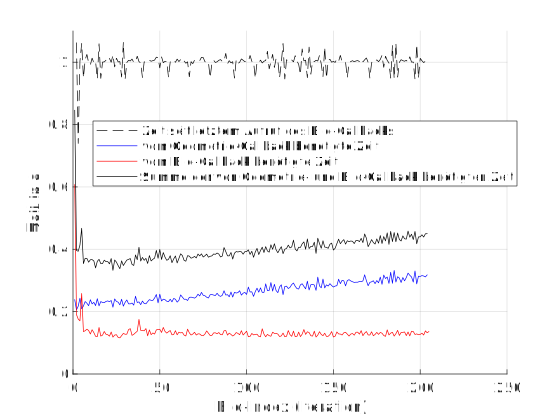
\includegraphics[width=0.7\textwidth]{evaluation_riverflow_times_combined_1Hz_0.1m_s_over_piciter}
	\label{fig:evaluation:riverflow:times_combined_1Hz_0.1m_s_over_piciter}
\end{figure}